\documentclass[12pt,oneside,a4paper,english]{article}
\usepackage[T1]{fontenc}
\usepackage[utf8]{inputenc} % Changed from latin2 to utf8 for better compatibility
\usepackage[margin=2.25cm,headheight=26pt,includeheadfoot]{geometry}
\usepackage[english]{babel}
\usepackage{listings}
\usepackage{color}
\usepackage{titlesec}
\usepackage{titling}
\usepackage[framed, numbered]{matlab-prettifier}
\usepackage{changepage}
\usepackage{amsmath}
\usepackage{hyperref}
\usepackage{enumitem}
\usepackage{graphicx}
\usepackage{fancyhdr}
\usepackage{lastpage}
\usepackage{caption}
\usepackage{tocloft}
\usepackage{setspace}
\usepackage{multirow}
\usepackage{titling}
\usepackage{float}
\usepackage{comment}
\usepackage{booktabs}
\usepackage{indentfirst}
\usepackage{lscape}
\usepackage{booktabs,caption}
\usepackage[flushleft]{threeparttable}
\usepackage[english]{nomencl}
\usepackage{xcolor}
\usepackage{lipsum}

% Set up hyperref
\hypersetup{
    colorlinks=true,
    linkcolor=blue,
    filecolor=magenta,      
    urlcolor=cyan,
    pdftitle={History of The Sun, Moon and Earth},
    pdfpagemode=FullScreen,
}

% --- set footer and header ---
\pagestyle{fancy}
\fancyhf{}
\rhead{History of The Sun, Moon and Earth}
\lhead{Astronomical Observation}
\author{}
% --- Title formatting ---
\title{\textbf{The Sun, Earth and Moon: A Cosmic Relationship}}
\date{\today}

% --- Fix typo in Aldebaran throughout document ---
\newcommand{\Aldebaran}{Aldebaran}

% --- End of page settings ---
\begin{document}
\maketitle

\begin{abstract}
    This document provides insight into the relationship between the Sun, Earth, and Moon. The sun serves as the center of our solar system, with Earth orbiting around it while the moon orbits Earth. While humanity has observed these celestial bodies for thousands of years, we've only recently come to fully understand their motions and physical properties. The sun's history began 4.6 billion years ago, and although human astronomical observation spans a much shorter timeframe, our journey of discovery continues to yield exciting new knowledge.
\end{abstract}

\section{Scientific Introduction to the Sun, Earth and Moon}
\subsection{Sun's Formation}
Newton's law of universal gravitation describes the gravitational force between two objects as:
\begin{equation}
    F = \frac{G \cdot m_1 \cdot m_2}{r^2}
\end{equation}
where $m_1$ and $m_2$ are the masses of the two objects, $r$ is the distance between their centers, and $G$ is the gravitational constant ($6.674\cdot 10^{-11} m^3 \cdot kg^{-1} \cdot s^{-2}$). When one body is significantly more massive than the other, gravity primarily depends on the larger object. This explains why Earth's gravity is typically understood as:
\begin{equation}
    F = \frac{G \cdot m_e}{r^2}
\end{equation}

Gravitational force maintains planetary orbits around the sun and lunar orbits around their planets. The sun's enormous mass creates sufficient gravitational pull to keep all solar system planets in orbit. This principle applies to smaller objects as well. Approximately 4.6 billion years ago, the sun began as a nebula of gas and dust particles. These particles attracted one another, gradually forming larger clumps through a process called accretion.

\begin{figure}[H]
    \centering
    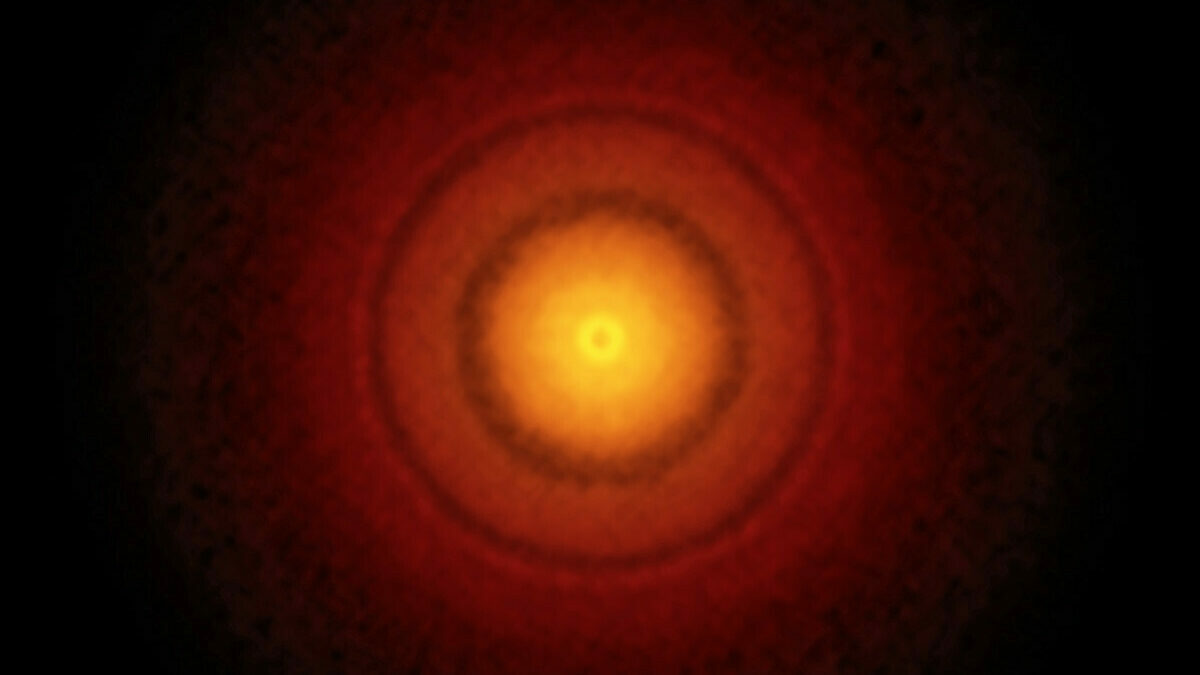
\includegraphics[width=0.8\textwidth]{SolarSys1.jpg}
    \caption{Image of an accretion disk surrounding a distant protostar. The dark bands represent paths where planets are forming within the dust clouds.\cite{solarsysImg}}
    \label{fig:solardisk}
\end{figure}

The nebula consisted primarily of hydrogen and helium, with trace amounts of other elements. Friction within the spinning accretion disk generated heat until the protostar began emitting light, though nuclear fusion had not yet commenced. As the star continued accumulating material, planets and moons formed through similar accretion processes. These bodies remained too small for fusion, becoming cooler than the star. All orbiting bodies continued gathering material until the protostar initiated hydrogen fusion, at which point it ejected surrounding dust to become a main sequence star.

This early period remained turbulent for the young solar system, with planets and planetesimals frequently colliding and scattering debris into chaotic orbits. During this chaotic era, Earth collided with a proto-planet named Theia\cite{moonformation}, an event that ultimately formed our moon.

\subsection{The Earth and Its Moon}
Earth's protoplanet began forming approximately 4.54 billion years ago as its accretion disk accumulated sufficient material to collapse into a roughly spherical shape. The sun's initiation of fusion ejected all dust not gravitationally bound to Earth. Nearby planets and planetesimals with intersecting orbits frequently collided with early Earth, resulting in a cosmic "bumper car" scenario where Earth either absorbed material from smaller impacts or lost material in collisions with similarly-sized bodies.

These collisions rendered Earth's surface extremely hot and molten. As the crust and mantle cooled, the Theia impact ejected portions of both bodies' mantles into space. This debris, captured by Earth's gravity, began orbiting our planet. As the solar system stabilized, both Earth's surface and the newly formed moon continued cooling.

The Earth and Moon share similar composition because the Moon originated from Earth's ejected material. The Moon lacks an atmosphere due to its smaller iron core, which generates an insufficient magnetic field to deflect solar wind. Earth's larger iron core produces a stronger magnetic field that protects our atmosphere. The Moon measures approximately one-quarter Earth's size with one-sixth its gravity. Together, they form the Earth-Moon system that orbits the sun.

\subsection{The Sun and Moon}
\subsubsection{Elliptical Orbits}
The moon orbits Earth in an elliptical (oval) path, as do all solar system orbits due to universal gravitation. Newton developed calculus to describe these motions, while Kepler established his three laws of planetary motion:
\begin{itemize}
    \item The Law of Orbits: All planets move in elliptical orbits with the sun at one focus.
    \item The Law of Areas: A line connecting a planet to the sun sweeps equal areas in equal times.
    \item The Law of Periods: The square of a planet's orbital period is proportional to the cube of its orbit's semi-major axis.\cite{kepler}
\end{itemize}

Regarding Earth and Moon, the Moon essentially orbits Earth like a planet with some unique characteristics.

\subsubsection{Tidal Locking}
Our Moon is tidally locked to Earth, meaning its rotation period matches its orbital period. This synchronization causes the same lunar hemisphere to always face Earth. Tidal locking results from gravitational differences between the Moon's near and far sides, creating a bulge that eventually stabilized the Moon's orientation. The Moon's gravitational influence also creates Earth's ocean tides.

\subsubsection{Eclipses}
Eclipses occur when celestial bodies align to block sunlight. A lunar eclipse happens when Earth blocks sunlight from reaching the Moon, while a solar eclipse occurs when the Moon blocks sunlight from reaching Earth. Lunar eclipses occur multiple times annually. The Moon's visibility results from reflected sunlight, and as it orbits Earth (completing a lunar cycle in approximately 28 days), it periodically enters Earth's shadow, becoming nearly invisible during the "new moon" phase. As the Moon emerges from shadow, reflected light increases its visibility.

\begin{figure}[H]
    \centering
    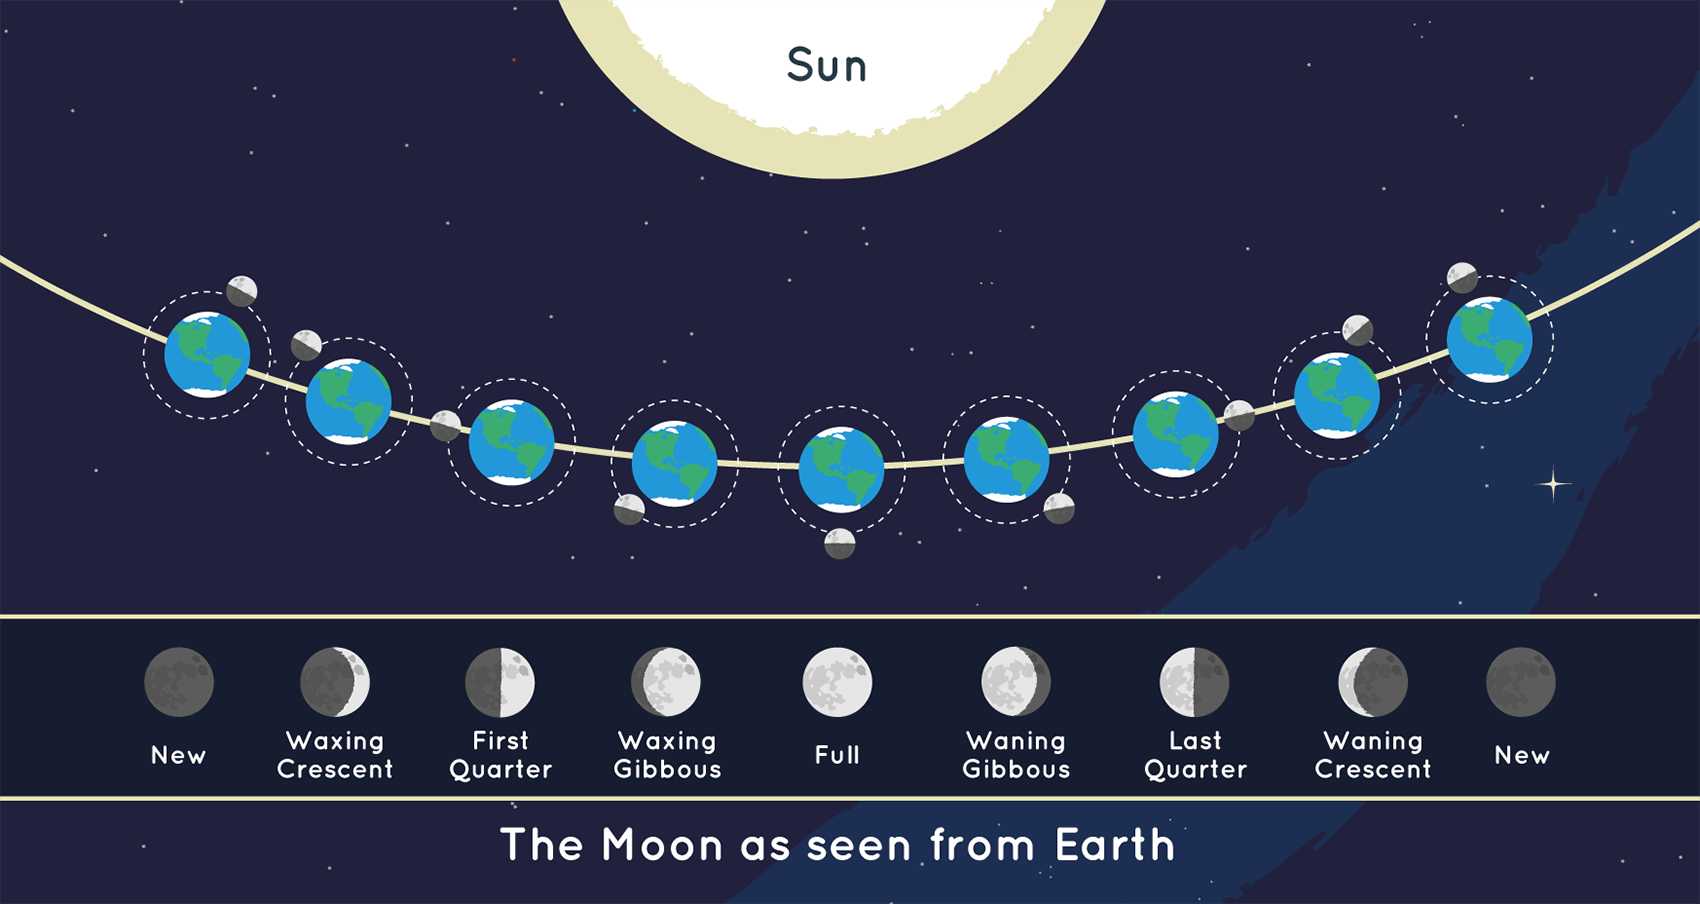
\includegraphics[width=0.8\textwidth]{moon-phases-jpl.png}
    \caption{The Moon's phases, showing how the new moon occurs when in Earth's shadow.\cite{moonphase}}
\end{figure}

Solar eclipses are rarer because the Moon's alignment between Earth and Sun occurs less frequently, and its shadow covers only a small portion of Earth. Eclipse observers measure visibility by "totality." Partial solar eclipses occur when the Moon blocks a portion of the Sun, while total solar eclipses completely obscure the Sun within a narrow (approximately 100-mile wide) path of totality. Note: sunlight around the eclipsed Sun remains dangerous to view directly. The next total solar eclipse occurs on August 12, 2026.

\section{History of Solar and Lunar Observation}
Humanity has observed the sun and moon for millennia, using them for timekeeping, navigation, and seasonal prediction. Ancient civilizations including the Babylonians, Chinese, and others tracked these celestial bodies for agricultural, religious, and commercial purposes.

As humans transitioned from nomadic to sedentary lifestyles, they established permanent farms near Mesopotamian rivers while developing astronomical knowledge. Early observers noted correlations between celestial positions and seasonal changes, initially measuring time by counting lunar cycles (approximately 29.5 days between new moons). This lunar calendar proved challenging due to difficulty spotting new moons and accumulated an 11-day annual discrepancy (354-day lunar year vs. 365-day solar year). Without correction, this discrepancy would shift seasons by about one month every three years - problematic for agricultural planning. Mesopotamian rulers implemented calendar adjustments to maintain alignment with planting and harvest cycles.\cite{meso1}

Ancient cultures often interpreted eclipses as omens, but some pursued scientific understanding. Babylonians achieved remarkable eclipse prediction accuracy by tracking celestial positions and performing mathematical calculations. They developed solar-lunar calendars superior to purely lunar systems. Greeks, Egyptians, and independently, Mayans continued advancing this astronomical knowledge.\cite{ancientobs}

While ancient civilizations often deified celestial bodies, they also recognized predictable, measurable patterns in their movements. These observations connected celestial events with terrestrial phenomena. Though lacking modern astrophysical knowledge (despite Greek understanding of Earth's sphericity), ancient astronomers established foundational relationships that persist in modern astronomy.

\section{Do We Know Everything about the Sun and Moon?}
While we certainly don't know everything, it's more productive to ask what specific mysteries remain regarding these celestial bodies.

\subsection{Current State of Solar and Lunar Observation}
We've physically visited the Moon through Apollo missions, returning samples for study. Lunar knowledge exceeds oceanic understanding because the Moon lacks atmosphere and weather. NASA plans renewed lunar missions, including potential long-term habitation to facilitate manufacturing and mining operations in the Moon's lower gravity.

The Moon's cratered surface results from its lack of atmospheric protection - unlike Earth, where most small asteroids (meteors) burn up in the atmosphere. We've also discovered subsurface water ice, offering clues about lunar formation and possible comet impacts. Lunar surface dust (regolith) differs significantly from terrestrial soil - its fine, sharp particles result from absent weathering processes. This abrasive regolith presents challenges for lunar construction and equipment durability.

\begin{figure}[H]
    \centering
    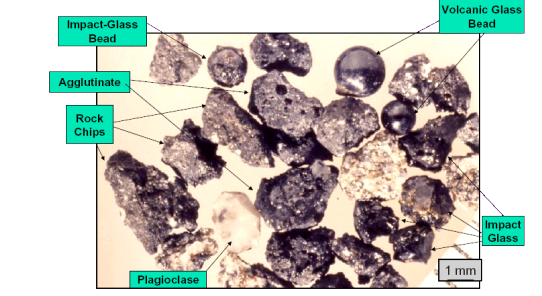
\includegraphics[width=0.8\textwidth]{Regolith.png}
    \caption{Regolith particles exhibiting sharp edges characteristic of unweathered lunar dust.\cite{regolith}}
    \label{fig:regolith}
\end{figure}

The Sun presents different observational challenges as a continuous nuclear furnace emitting energy and plasma. Solar winds - streams of charged particles - create aurorae but can damage satellites. NASA monitors solar activity to predict these space weather events and protect sensitive electronics. Specialized satellites reveal sunspots - cooler surface regions caused by magnetic fluctuations. Like turbulent water, these fluctuations sometimes eject solar plasma in coronal mass ejections that could harm unprotected organisms and technology.\cite{sunspots}

\subsection{Mysteries of the Sun and Moon}
The Moon's origin remains its greatest mystery. While the Theia impact theory predominates, uncertainties persist. We're also uncertain about subsurface water quantity and distribution.

The Moon gradually recedes from Earth at about 1 inch annually. Over billions of years, this will eliminate lunar tides and eventually release the Moon from Earth's orbit - a process whose consequences remain mysterious.

Contrary to popular imagination, the Moon's "dark side" (more accurately, its far side) isn't fundamentally mysterious. Soviet Luna 3 first imaged it in 1959, revealing more craters and barren landscape. However, a massive far-side crater exposes deep lunar crust material giving more insight into the amount of water under the crust.\cite{darkmoon}

\begin{figure}[H]
    \centering
    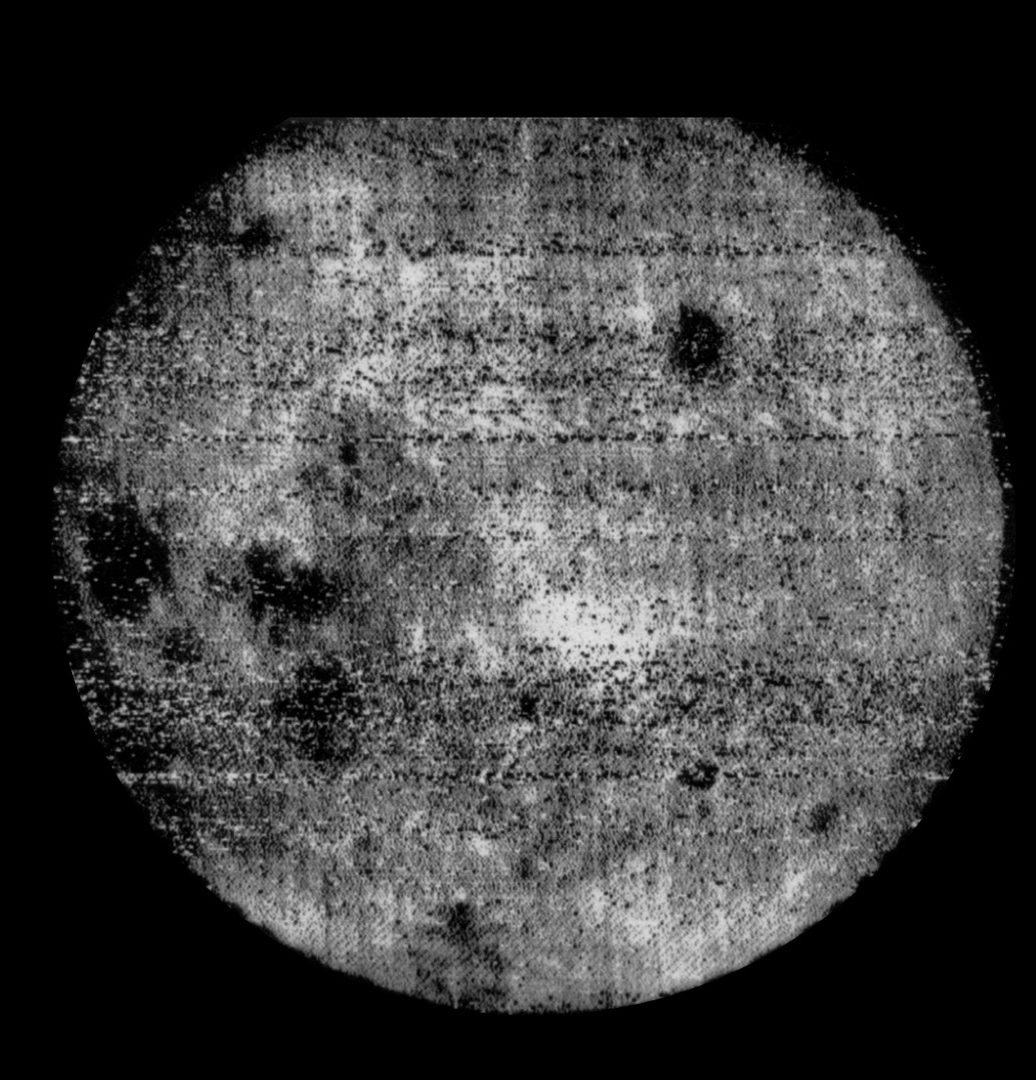
\includegraphics[width=0.6\textwidth]{DarkMoon.jpg}
    \caption{The Moon's far side as imaged by Luna 3.\cite{darkmoon}}
    \label{fig:darkmoon}
\end{figure}

\subsection{Future of Solar and Lunar Observation}
NASA's Parker Solar Probe recently achieved the closest solar approach (3.8 million miles), providing unprecedented data about solar surface dynamics and magnetic fields. Continued solar observation will enhance our understanding of fusion and stellar evolution across the Sun's 10-billion-year lifespan.

As humanity expands into space, the Moon will likely become a practical stepping stone for spacefaring development.

\newpage
\section{References}
\bibliography{OrbitalMech.bib}
\bibliographystyle{ieeetr}
\end{document}